\documentclass[12pt, oneside]{article}
\usepackage{bookmark}
\usepackage{graphicx}
\usepackage{hyperref}
\graphicspath{{images/}}
\begin{document}
 
%titlepage
\thispagestyle{empty}
\begin{center}
\begin{minipage}{0.75\linewidth}
    \centering
%University logo
    
\includegraphics{UPlogo}
    \rule{0\linewidth}{0.15\linewidth}\par

%Thesis title
    {\uppercase{\Large Functional Requirements\par}}
   	{\uppercase{\Large cos 301 group 2 b \par}}
    \vspace{1cm}
%Author's name
    {\normalsize Byron Dinkelmann u11057638\par}
    {\normalsize Johan van Rooyen u11205131\par}
    {\normalsize Mandla Mhlongo u29630135\par}
    {\normalsize Ryno Pierce u12003922\par}
    {\normalsize Sylvester Mpungane u11241617\par}
    {\normalsize Molefe Molefe u12260429\par}
    {\normalsize Taariq Ghoord u10132806\par}
    {\normalsize Timothy Snayers u13397134\par}
    \vspace{1cm}
    
    \hyperref[https://github.com/ByronDinkelmann/COS-301-Group-2-b.git]{Github}\par
    \vspace{1cm}
%Date
    {\Large February 2015}
\end{minipage}
\end{center}
\clearpage

\tableofcontents
\newpage

\section{Introduction}
This document outlines the functional requirements of "The Computer Science Education Didactic and Applications Research"(CSEDAR) registered research project called "The use of Online Discussion in Teaching"(TODT). This document describes the "Buzz" system to be developed and gives insight to how to achieve this implementation for those implementing it. 
\section{Vision}
The research projects aim is to find ways to enhance and improve the learning of students with the use of online discussion. This online forum "Buzz" will become part of the Computer Science websites modules, creating an online space for discussion for each or where relevant. Where students, teaching assistants and lecturers can engage in activities
related to learning the content of the specific module while applying game concepts to motivate students to increase the quality of their participation and consequently experience deeper learning of the course content. 
\section{Background}
The reason for this research project is the problem of engaging an extremely large number of first year students within The University of Pretoria, specifically the Computer Science Department students. Currently available tools for discussion forums lead to the problems that are hampering positive engagement of teaching staff and students. These problems consist of inexperienced users, unorganized content and low levels of excitement.
To combat these problems the "Buzz" system intends to have the basic functionality of online forums, have automated feedback on common mistakes, have a Game-like presentation and have automated structuring.

The University of Pretoria have the opportunity to teach the COS301 "Software Engineering" students while being able to improve current systems of online discussion which can be extended to benefit all students in the future. 

The research project gives the students of COS301 "Software Engineering" an opportunity to learn form the experiences of designing, creating and developing this system, which include learning to work with colleagues, creating documentation, simplifying and improving the communication of lectures and students through a structured forum, using online systems for group work and the basic process of how software is designed, created and developed in business to name but a few.
\section{Functional Requirements and application design}

\subsection{Purpose}
\begin{enumerate}
 \item{CRUD}: To create posts on the buzz system so that users in the system can share relevant information with one another and communicate. To allow registered users and non registered users such as guests to view posts created by users of the buzz system. To allow users to update posts of which they control. To allow users to delete their own posts or to allow users with sufficient status level to delete other posts based on certain factors about that specific post.
 \\
\item{Message Restrictions}: To restrict users to length, content and positioning of posts based on the users status level. 
\\
 \item{Message Tracker}: To mark posts for each registered user so that they can keep track of which posts they have read and which users have read certain posts.
\\
 \item{Thread Summarizer}: To summarize threads, that are over a certain number of posts long, into a new thread for viewing. This replaces the original thread.
\\
 \item{Template Messenger}: To give standard and custom layouts of automated messages that can be broadcast to groups or sent to individuals.
\\
\item{Check Post For Plagiarism}: To use a service provider to check if a post has been plagiarised.
\\
\item{Report Post For Plagiarism}: To enable users to be able to report posts that they suspect is plagiarised (with a link to the original), because the system couldn't detect it.
\\
\item{Netiquette}: To ensure that every post submitted conforms with the netiquette rules.
\\
%%%%%%Taariq%%%%%%%%%%
\item{Text decorating functions}: To allow privileged users to use advanced functions when typing posts.
\\
\item{Statistical gathering}:To advance users to their next level for gamification concept.
\\
%%%%%%Taariq%%%%%%%%%%

 
\end{enumerate}

\subsection{Use case prioritization}
\subsubsection{CRUD}
Critical
\subsubsection{Message Restrictions}
Critical
\subsubsection{Message Read Tracker}
Important
\subsubsection{Thread Summarizer}
Nice-to-have
\subsubsection{Template Messenger}
Nice-to-have
\subsubsection{Check Post For Plagiarism}
Nice To Have
\subsubsection{Report Post For Plagiarism}
Nice To Have
\subsubsection{Netiquette}
Nice To Have
%%%%%%Taariq%%%%%%%%%%
\subsubsection{Text Decorating}
Nice To Have
\subsubsection{Statistical gathering}
Critical
%%%%%%Taariq%%%%%%%%%%


\subsection{Use case/Service contracts}
\subsubsection{CRUD}
\begin{enumerate}
 \item Pre-conditions for CRUD: The buzz system needs to be available and a connection to the buzz system possible.
 
  \item Request and Result Data Structures: \\
 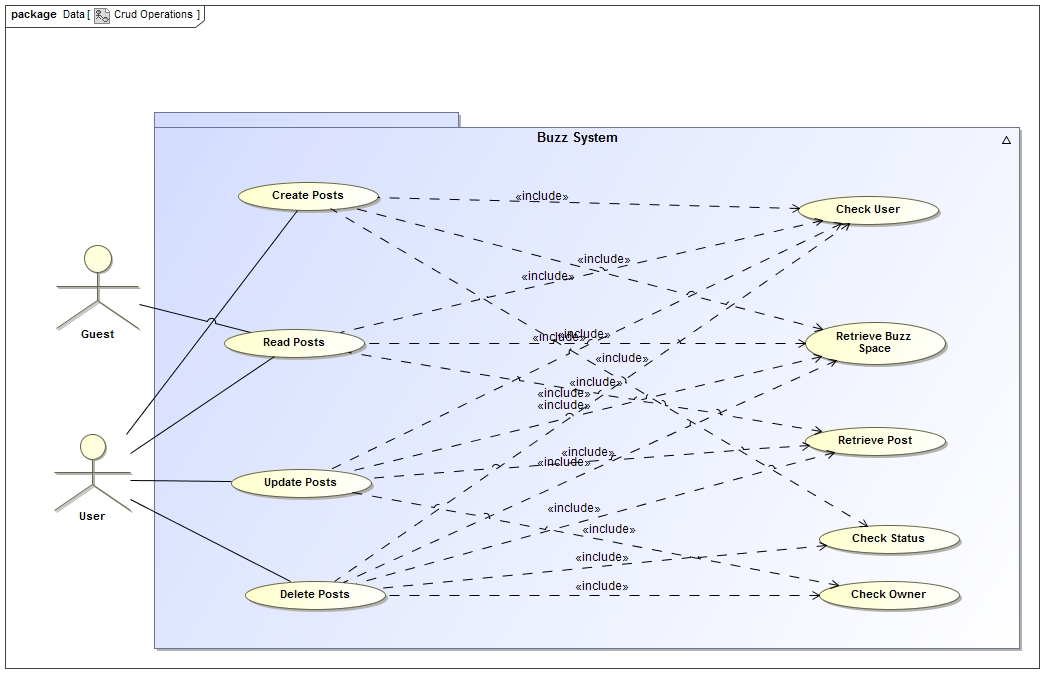
\includegraphics[scale=0.3]{CRUDOperations}\\
 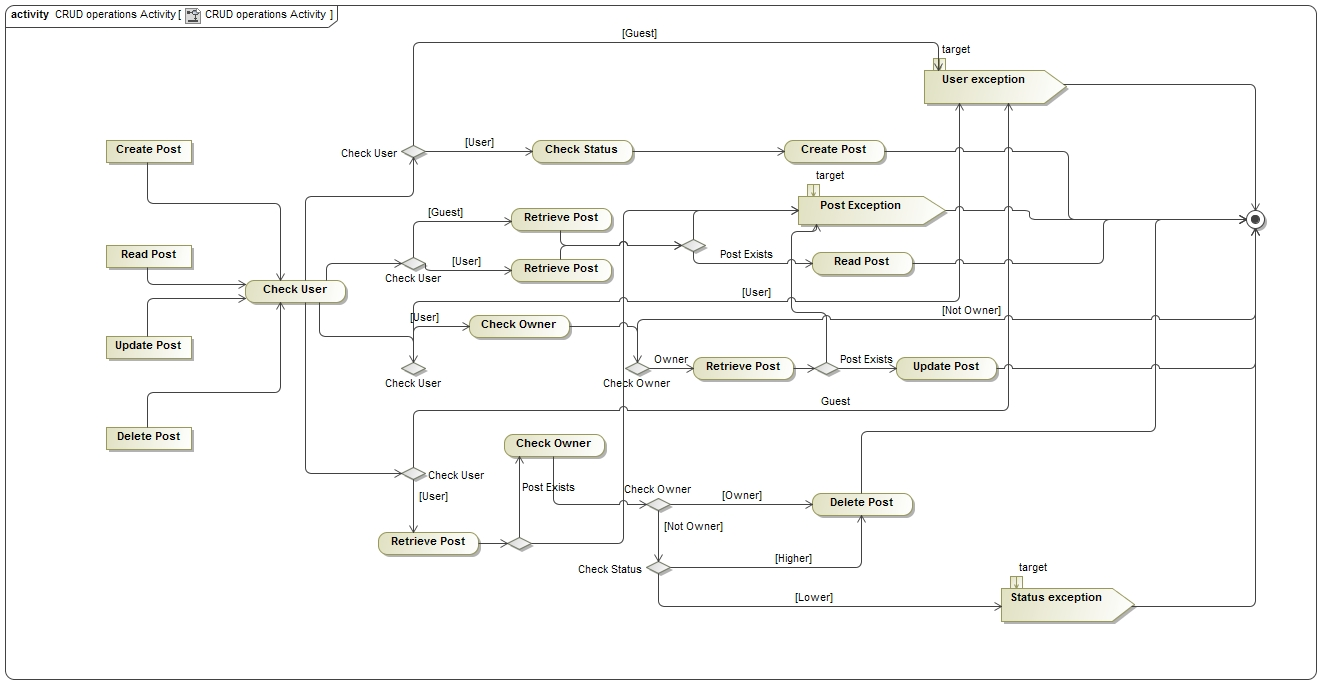
\includegraphics[scale=0.3]{CRUDOperationsActivity} 
\end{enumerate}
\subsubsection{CRUD-Create}
\begin{enumerate}
 \item Pre-conditions: For a user to create posts they need to be registered of the buzz system. The user must be logged in to the buzz system.
 \\
 \item Post-conditions: Posts will succeed to be created and will appear in the buzz system where posted.
  \\
 
\end{enumerate}


%%%%%%%%%%%%Taariq%%%%%%%%%%%%%%%%
\subsubsection{Text Decorating}
\begin{enumerate}
 \item Pre-conditions: User must have required level.
 \\
 
\item Post-conditions: User can use the pretty text functionality that he/she qualifies for. 
\\  
  
 \item Request and Result Data Structures:\\
  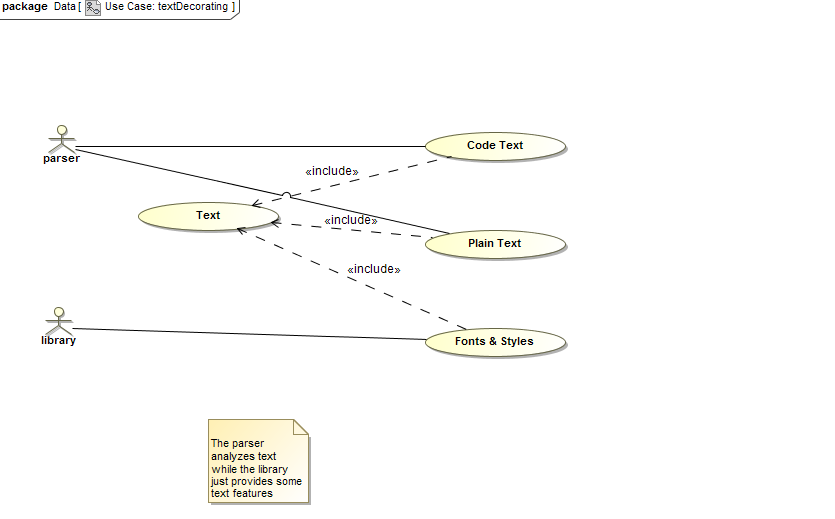
\includegraphics[scale=0.4]{textDecorator}\\
 \item Request and Result Data Structures:\\
  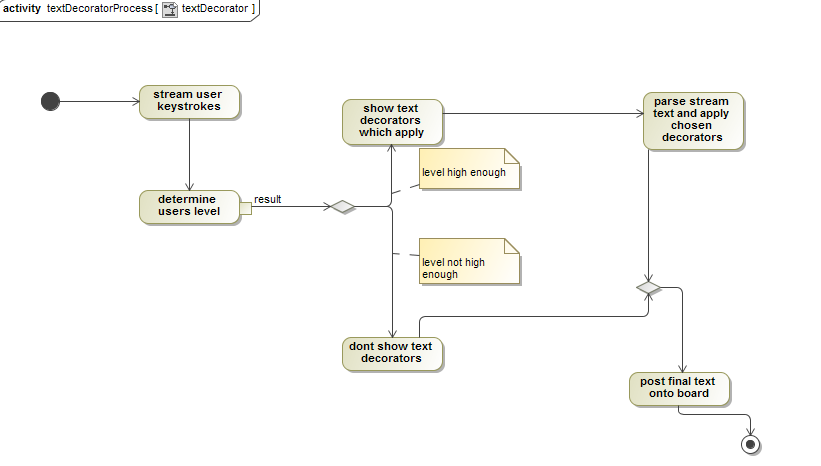
\includegraphics[scale=0.4]{textDecoratorProcess}\\


\end{enumerate}
%%%%%%%%%%%%%%%%Taariq%%%%%%%%%%%%%%%%%%%%

%%%%%%%%%%%%Taariq%%%%%%%%%%%%%%%%
\subsubsection{Statistical Gathering}
\begin{enumerate}
 \item Pre-conditions: Database must be up and accessible.
 \\
 \item Users want to level up to use privileged mechanisms 
\\

\item Post-conditions: Users who are students marks can be used to extract statistical information and these information can then be compared.
\\  
  \item users have leveled up.
  \\
  
 \item Request and Result Data Structures:\\
  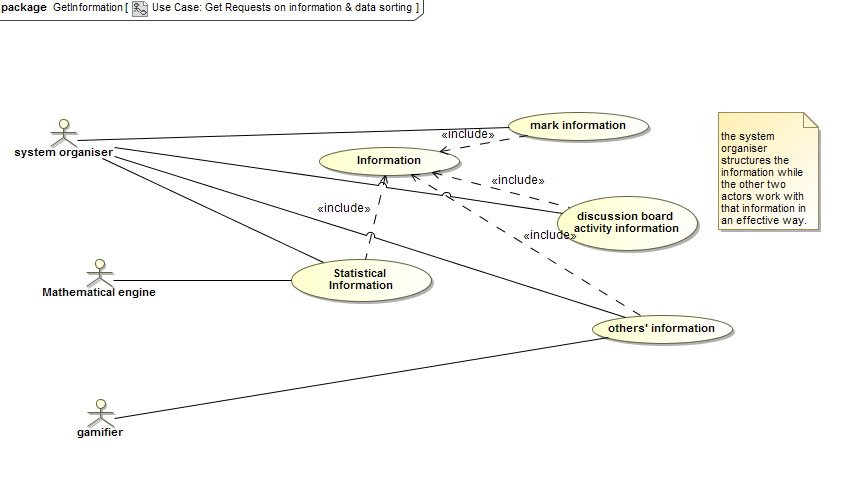
\includegraphics[scale=0.4]{getInformation}\\

\end{enumerate}
%%%%%%%%%%%%%%%%Taariq%%%%%%%%%%%%%%%%%%%%



\subsubsection{CRUD-Read}
\begin{enumerate}
 \item Pre-conditions: Posts must be present to be read.
 \\
 \item Post-conditions: Once a post has been viewed by a logged in registered user, the post should be marked as read for that specific user.
  \\

\end{enumerate}



\subsubsection{CRUD-Update}
\begin{enumerate}
 \item Pre-conditions:  For a user to update posts they need to be registered of the buzz system. The user must be logged in to the buzz system. The user must be the owner of the post.
 \\
 \item Post-conditions: Post will be updated and shown on the buzz system to be updated.
   \\

\end{enumerate}

\subsubsection{CRUD-Delete}
\begin{enumerate}
 \item Pre-conditions:  For a user to delete posts they need to be registered of the buzz system. The user must be logged in to the buzz system. The user must be the owner of the post unless a user with status level "x" views the post to be unfit. The post needs to exist for it to be deleted.
 \\
 \item Post-conditions: Post successfully deleted will be hidden from the other users and buzz system and archived.Posts will never be physically deleted from the system itself.
   \\

\end{enumerate}

\subsubsection{Message Restrictions}
\begin{enumerate}
 \item Pre-conditions:  User must be registered on the buzz system. The buzz system needs to be available and a connection to the buzz system possible. The user must be logged in to the buzz system. User must be able to create posts. Length and content of posts must be specified by the buzz system of which the user is registered. Must have levels of posts.
 
 \item Post-conditions: Post will be created and shown on the buzz system. Correct length and content of posts if buzz system is configured correctly.
   \\
 \item Request and Result Data Structures:\\
  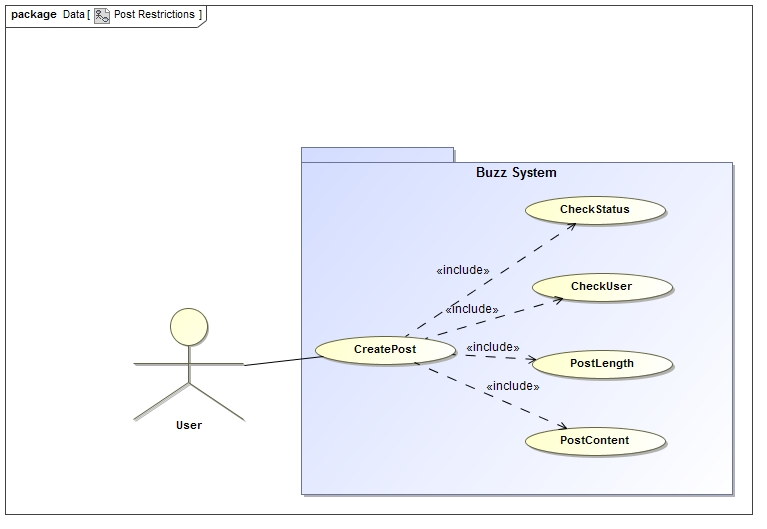
\includegraphics[scale=0.4]{PostRestrictions}\\
 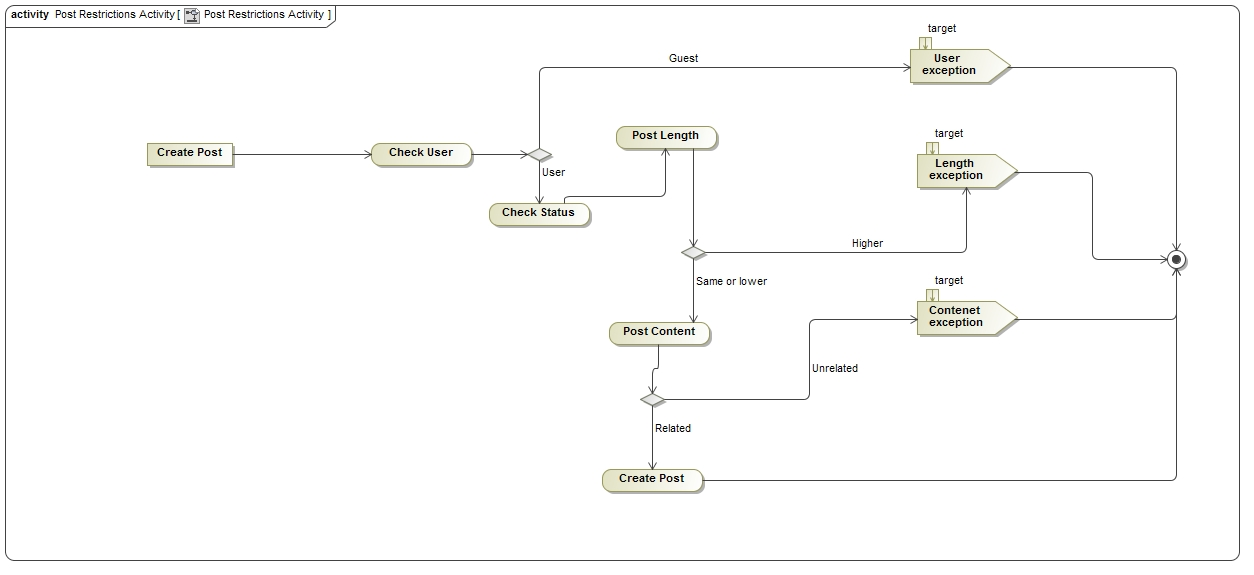
\includegraphics[scale=0.35]{PostRestrictionsActivity} 
\end{enumerate}

\subsubsection{Message Read Tracker}
\begin{enumerate}
 \item Pre-conditions:  User must be registered on the buzz system. The user must be logged in to the buzz system. Messages must exist to be read, marked as unread and must be seen as read by other users.
 \\
 \item Post-conditions: Post is marked as unread.Post is marked when read and seen to be read on the buzz system.
   \\
 \item Request and Result Data Structures:\\
   \includegraphics[scale=0.4]{PostReadTracker}\\
 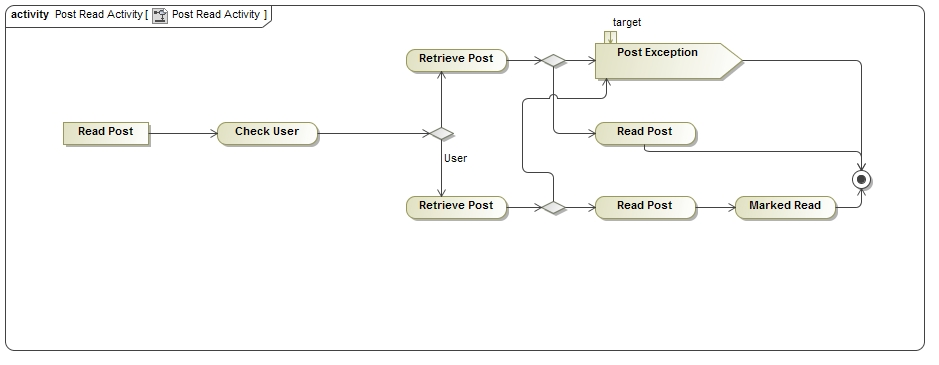
\includegraphics[scale=0.4]{PostReadActivity} 
\end{enumerate}
\subsubsection{Thread Summarizer}
\begin{enumerate}
 \item Pre-conditions:  The user must be registered on the buzz system. The buzz system must be on-line and reachable and the user must be logged in. Only high level users can summarize threads.
 \item Post-condition:  The summarized thread will be viewable on the buzz system on the relevent buzz space. The original thread will be hidden from view.
 \\
\item Request and Result Data Structures:\\
   \includegraphics[scale=0.4]{ThreadSummarizer}\\
 \includegraphics[scale=0.4]{ThreadSummarizerActivity} 
\end{enumerate}
\subsubsection{Template Messenger}
\begin{enumerate}
\item Pre-conditions:   The buzz system must be on-line and reachable. Since this procedure is automated a user does not need to be logged in.
\item Post-conditions:  The message(s) must be sent. The message(s) must be delivered to the recipient(s).
\\
\item Request and Result Data Structures:\\
   \includegraphics[scale=0.4]{TemplateMessenger}\\
 \includegraphics[scale=0.4]{TemplateMessengerActivity} 
\end{enumerate}
\subsection{Functions To Apply Social Tagging}
\begin{enumerate}
\item The system will provide functions which through employing tags can provide flexible ways of using information that supports users with: Finding, Collecting, Storing, Organizing and Sharing Information.
\item Allow users to share their tags.
\item Allow users different views of the content. Either a personally structured view according to the user's tags or the default admin structure.
\end{enumerate}
\subsection{Apply Self-Organization}
\begin{enumerate}
\item The system will allow the user to organize their content themselves based on their social tags.
\item The system will allow the user to chose from different types of views either the base owns or public structure.
\end{enumerate}
\subsection{Pre-conditions}
\subsubsection{Social Tagging Functions}    
\begin{enumerate}
\item User is signed in and has default privileges to execute all social tagging functions functions.
\item User has already created tags before they can share them.
\item  System allows for different views of the content.
\end{enumerate}
\subsection{Self-Organization Based On Social Tagging}
\begin{enumerate}
\item Have three different structures users can choose from for viewing.
\end{enumerate}
\subsection{Post-conditions}
\subsubsection{Social Tagging Functions}    
\begin{enumerate}
\item After the user has executed any of the functions the user state changes.
\item After the user selects their view structure, the structure must stay consistent until the user chooses otherwise.
\end{enumerate}
\subsection{Self-Organization Based On Social Tagging}
\begin{enumerate}
\item After the user selects their view type, provide option to still be able to switch views.
\item Content must be displayed according to user's desire.
\end{enumerate}
\subsection{Use Cases}
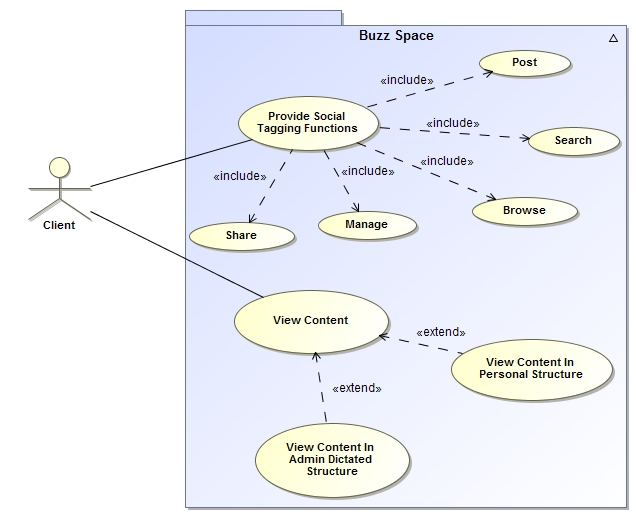
\includegraphics{socialTagging.jpg}
	\rule{0\linewidth}{0.15\linewidth}\par
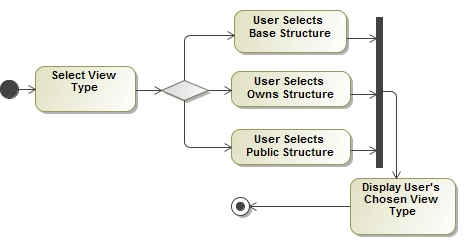
\includegraphics{socialTaggingActivity.jpg}
	\rule{0\linewidth}{0.15\linewidth}\par

\subsubsection{Changing User Status}
\begin{enumerate}
\item Description: The Buzz system will automatically rank users of the system based on their participation. A user's  reputation (status) will be affected by the user's participation points on Buzz system, it can either grow or be negatively affected depending on the user's participation marks.   
\item Actors: This functionality will be automatically triggered by the Buzz system each time a user's participation is evaluated.
\item Preconditions: The user needs to earn new participation points (positive or negative).
\item Post Conditions: The user's status should correspond to the status which the user's participation point maps to.
\item Request and Result Data Structure:
\begin{center}
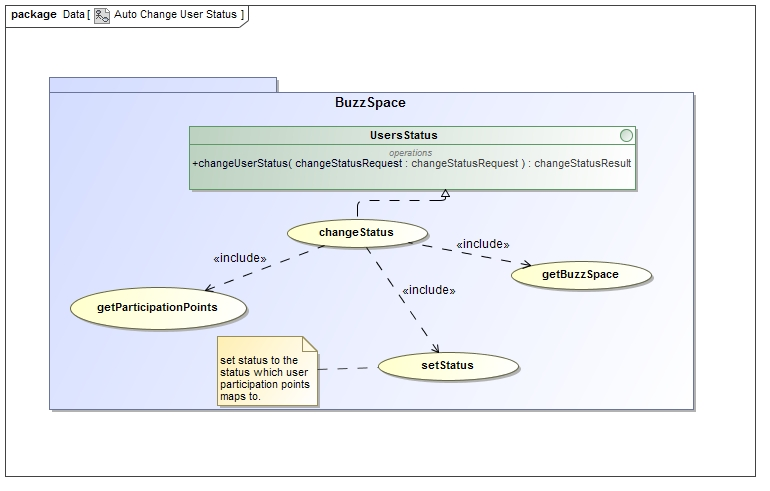
\includegraphics[scale=0.5]{AutoChangeUserStatus.jpg}
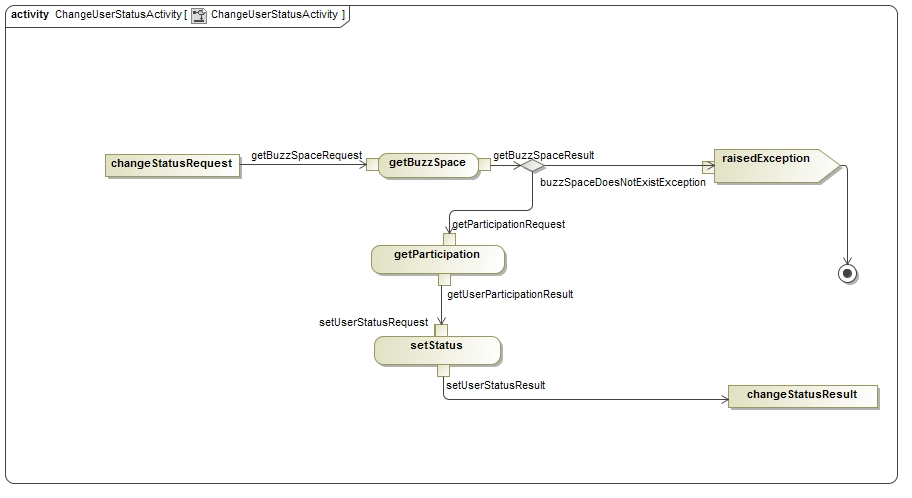
\includegraphics[scale=0.5]{ChangeUserStatusActivity.jpg}
\end{center}
\end{enumerate}

\subsubsection{System with Any Specified Host}
\begin{enumerate}
\item Description: The system should have the ability to be hosted by any site that it specified on setup by the administrator of the system the first time it is setup.
\item Actors: The administrator of the host site is the only user that can use this functionality to integrate the system on a site.
\item Preconditions: The user must be the site administrator and the host site specified must be a valid site.
\item Post Conditions: The system should be integrated on the site.
\item Request and Result Data Structure : 
\begin{center}
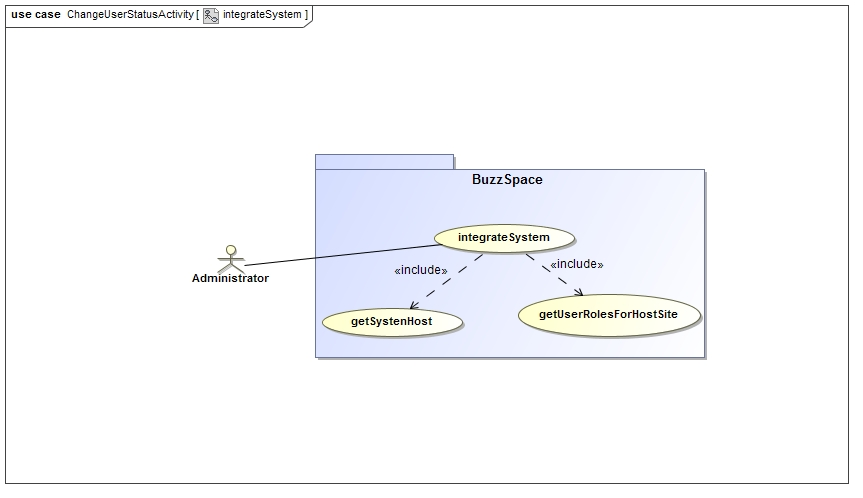
\includegraphics[scale=0.5]{integrateSystem.jpg}
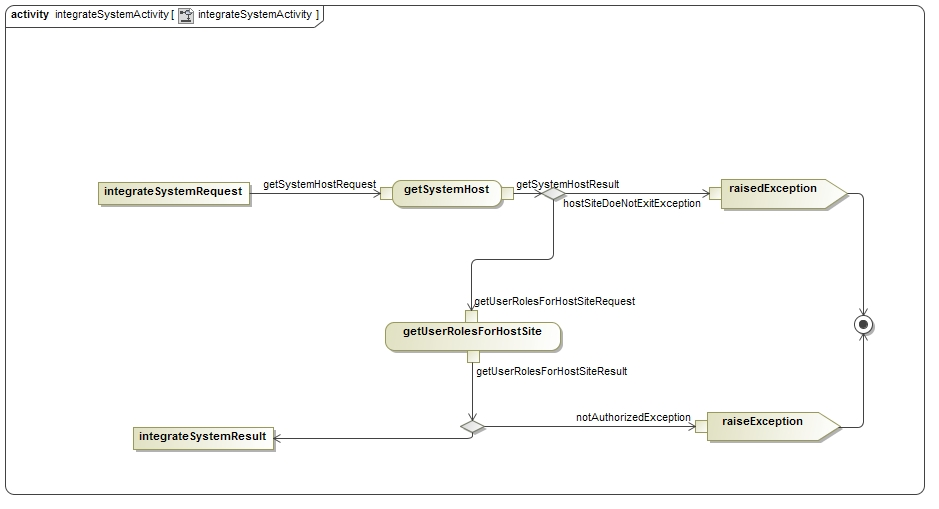
\includegraphics[scale=0.5]{integrateSystemActivity.jpg}
\end{center}
\end{enumerate}

\subsubsection{Check Post For Plagiarism}
\begin{enumerate}
 \item Pre-conditions: A post must have been submit by a registered user. 
 \\
 
 \item Post-conditions: If the post passes the plagiarism test, the new post should be registered on the system. If the post has failed the plagiarism tests the post will be blocked, then the post's user and the module's administrator will be notified. Afterwords a log will be stored. 
   \\
 \item Request and Result Data Structures:\\
  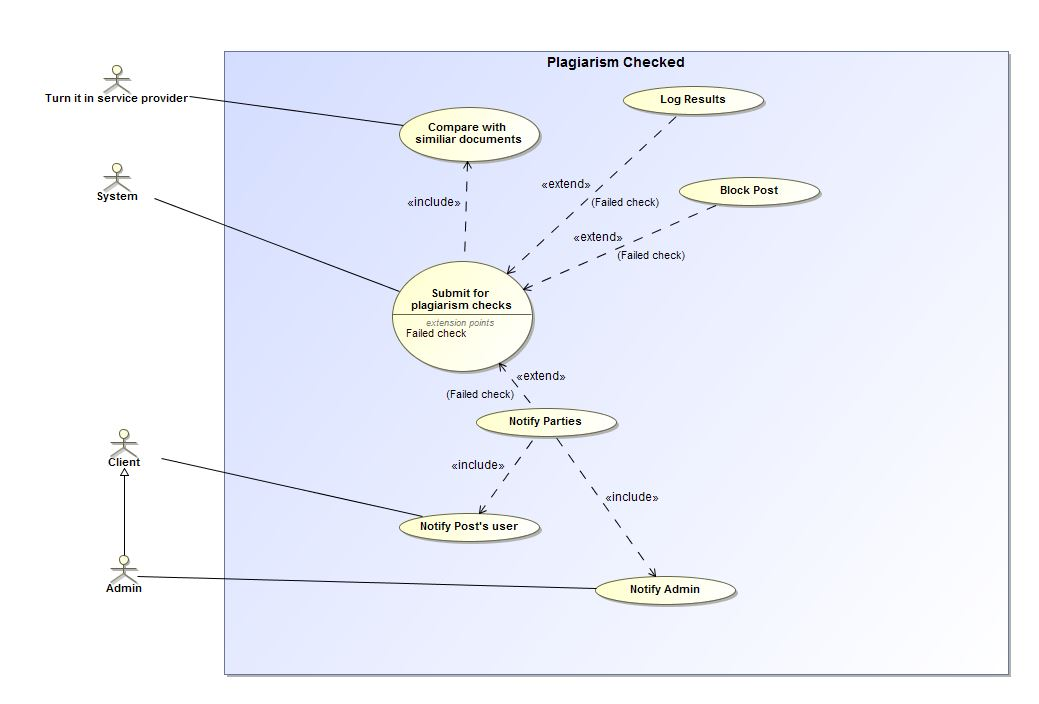
\includegraphics[scale=0.4]{plagiarismCheckUC}\\
 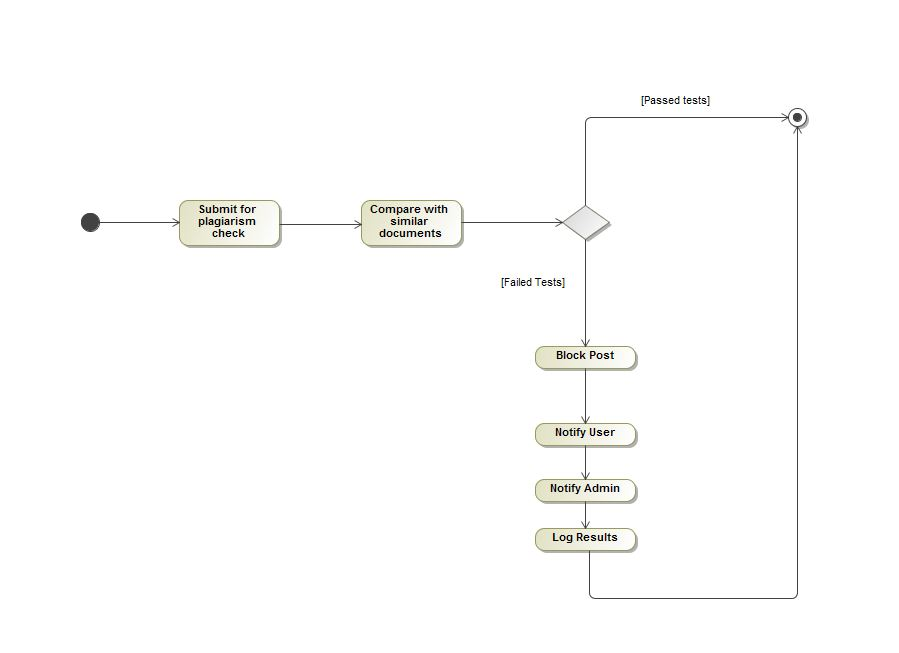
\includegraphics[scale=0.35]{plagiarismCheckAD} 
\end{enumerate}

\subsubsection{Report Post For Plagiarism}
\begin{enumerate}
 \item Pre-conditions: A post must have been reported by a registered user that has a level X account. 
 \\
 
 \item Post-conditions: The post is sent to an administrator to follow up on the report. If the administrator finds the post not plagiarised, the post will be registered on the system. If it is found to be plagiarised the post will be blocked, then the post's user and the module's administrator will be notified. Afterwords a log will be stored. 
   \\
 \item Request and Result Data Structures:\\
  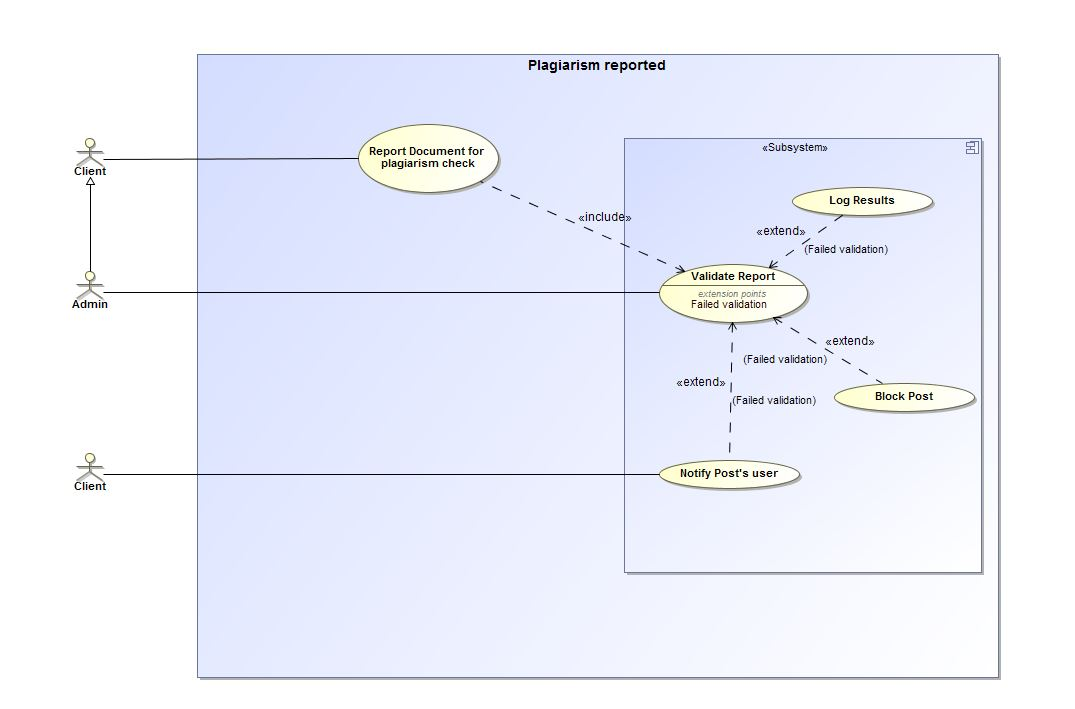
\includegraphics[scale=0.4]{plagiarismReportUC}\\
 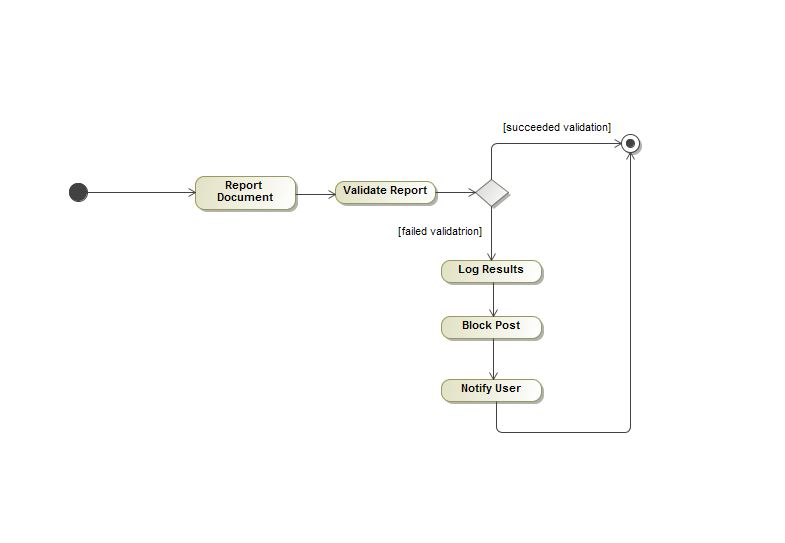
\includegraphics[scale=0.35]{plagiarismReportAD} 
\end{enumerate}


\subsubsection{Netiquette}
\begin{enumerate}
 \item Pre-conditions: A post must have been submit by a registered user.
 \\
 
 \item If the post passes the netiquette test, the new post should be registered on the system. If the post has failed the netiquette tests the post will be blocked, then the post's user and the module's administrator will be notified. Afterwords a log will be stored.  
   \\
 \item Request and Result Data Structures:\\
  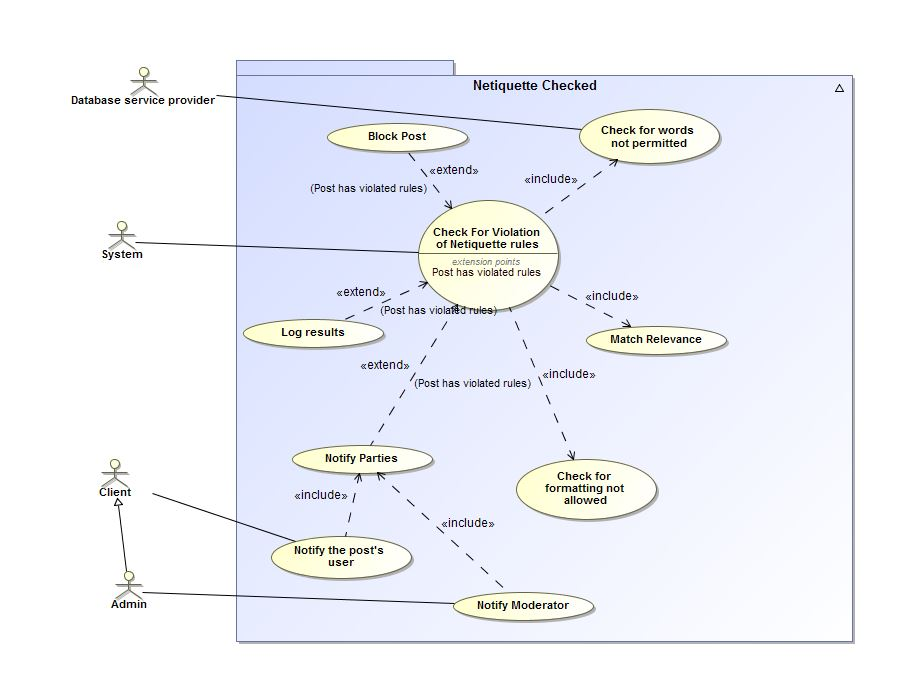
\includegraphics[scale=0.4]{netiquetteUseCase}\\
 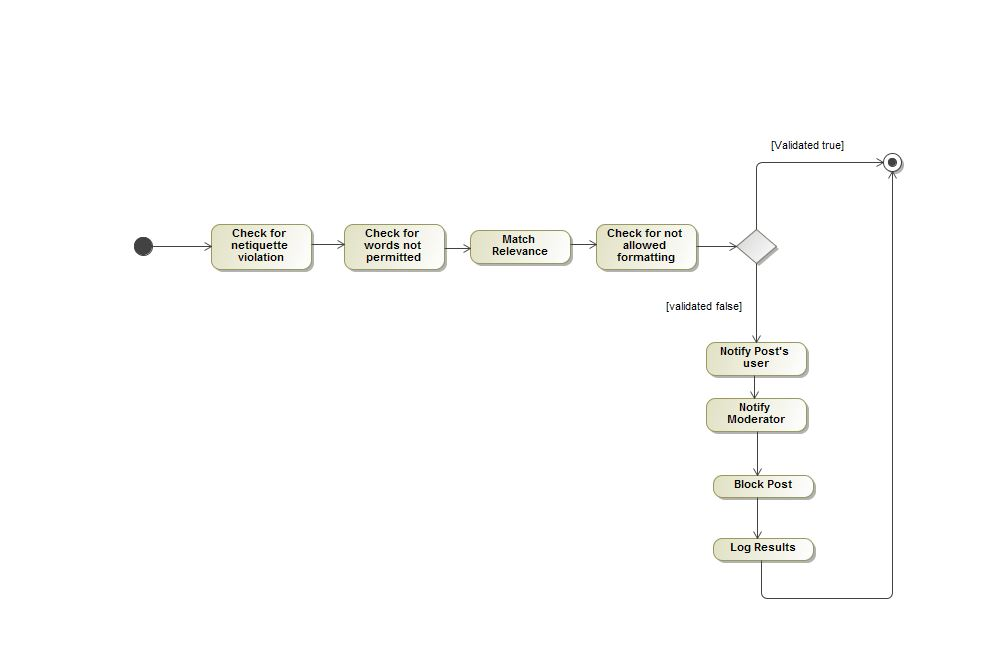
\includegraphics[scale=0.35]{NetiquetteActivityDiagram} 
\end{enumerate}

\subsection{Required functionality}
\subsection{Process specifications}
\subsection{Domain Model}
\section{Open Issues}


  
\end{document}
